\documentclass[1p]{elsarticle_modified}
%\bibliographystyle{elsarticle-num}

%\usepackage[colorlinks]{hyperref}
%\usepackage{abbrmath_seonhwa} %\Abb, \Ascr, \Acal ,\Abf, \Afrak
\usepackage{amsfonts}
\usepackage{amssymb}
\usepackage{amsmath}
\usepackage{amsthm}
\usepackage{scalefnt}
\usepackage{amsbsy}
\usepackage{kotex}
\usepackage{caption}
\usepackage{subfig}
\usepackage{color}
\usepackage{graphicx}
\usepackage{xcolor} %% white, black, red, green, blue, cyan, magenta, yellow
\usepackage{float}
\usepackage{setspace}
\usepackage{hyperref}

\usepackage{tikz}
\usetikzlibrary{arrows}

\usepackage{multirow}
\usepackage{array} % fixed length table
\usepackage{hhline}

%%%%%%%%%%%%%%%%%%%%%
\makeatletter
\renewcommand*\env@matrix[1][\arraystretch]{%
	\edef\arraystretch{#1}%
	\hskip -\arraycolsep
	\let\@ifnextchar\new@ifnextchar
	\array{*\c@MaxMatrixCols c}}
\makeatother %https://tex.stackexchange.com/questions/14071/how-can-i-increase-the-line-spacing-in-a-matrix
%%%%%%%%%%%%%%%

\usepackage[normalem]{ulem}

\newcommand{\msout}[1]{\ifmmode\text{\sout{\ensuremath{#1}}}\else\sout{#1}\fi}
%SOURCE: \msout is \stkout macro in https://tex.stackexchange.com/questions/20609/strikeout-in-math-mode

\newcommand{\cancel}[1]{
	\ifmmode
	{\color{red}\msout{#1}}
	\else
	{\color{red}\sout{#1}}
	\fi
}

\newcommand{\add}[1]{
	{\color{blue}\uwave{#1}}
}

\newcommand{\replace}[2]{
	\ifmmode
	{\color{red}\msout{#1}}{\color{blue}\uwave{#2}}
	\else
	{\color{red}\sout{#1}}{\color{blue}\uwave{#2}}
	\fi
}

\newcommand{\Sol}{\mathcal{S}} %segment
\newcommand{\D}{D} %diagram
\newcommand{\A}{\mathcal{A}} %arc


%%%%%%%%%%%%%%%%%%%%%%%%%%%%%5 test

\def\sl{\operatorname{\textup{SL}}(2,\Cbb)}
\def\psl{\operatorname{\textup{PSL}}(2,\Cbb)}
\def\quan{\mkern 1mu \triangleright \mkern 1mu}

\theoremstyle{definition}
\newtheorem{thm}{Theorem}[section]
\newtheorem{prop}[thm]{Proposition}
\newtheorem{lem}[thm]{Lemma}
\newtheorem{ques}[thm]{Question}
\newtheorem{cor}[thm]{Corollary}
\newtheorem{defn}[thm]{Definition}
\newtheorem{exam}[thm]{Example}
\newtheorem{rmk}[thm]{Remark}
\newtheorem{alg}[thm]{Algorithm}

\newcommand{\I}{\sqrt{-1}}
\begin{document}

%\begin{frontmatter}
%
%\title{Boundary parabolic representations of knots up to 8 crossings}
%
%%% Group authors per affiliation:
%\author{Yunhi Cho} 
%\address{Department of Mathematics, University of Seoul, Seoul, Korea}
%\ead{yhcho@uos.ac.kr}
%
%
%\author{Seonhwa Kim} %\fnref{s_kim}}
%\address{Center for Geometry and Physics, Institute for Basic Science, Pohang, 37673, Korea}
%\ead{ryeona17@ibs.re.kr}
%
%\author{Hyuk Kim}
%\address{Department of Mathematical Sciences, Seoul National University, Seoul 08826, Korea}
%\ead{hyukkim@snu.ac.kr}
%
%\author{Seokbeom Yoon}
%\address{Department of Mathematical Sciences, Seoul National University, Seoul, 08826,  Korea}
%\ead{sbyoon15@snu.ac.kr}
%
%\begin{abstract}
%We find all boundary parabolic representation of knots up to 8 crossings.
%
%\end{abstract}
%\begin{keyword}
%    \MSC[2010] 57M25 
%\end{keyword}
%
%\end{frontmatter}

%\linenumbers
%\tableofcontents
%
\newcommand\colored[1]{\textcolor{white}{\rule[-0.35ex]{0.8em}{1.4ex}}\kern-0.8em\color{red} #1}%
%\newcommand\colored[1]{\textcolor{white}{ #1}\kern-2.17ex	\textcolor{white}{ #1}\kern-1.81ex	\textcolor{white}{ #1}\kern-2.15ex\color{red}#1	}

{\Large $\underline{12a_{0929}~(K12a_{0929})}$}

\setlength{\tabcolsep}{10pt}
\renewcommand{\arraystretch}{1.6}
\vspace{1cm}\begin{tabular}{m{100pt}>{\centering\arraybackslash}m{274pt}}
\multirow{5}{120pt}{
	\centering
	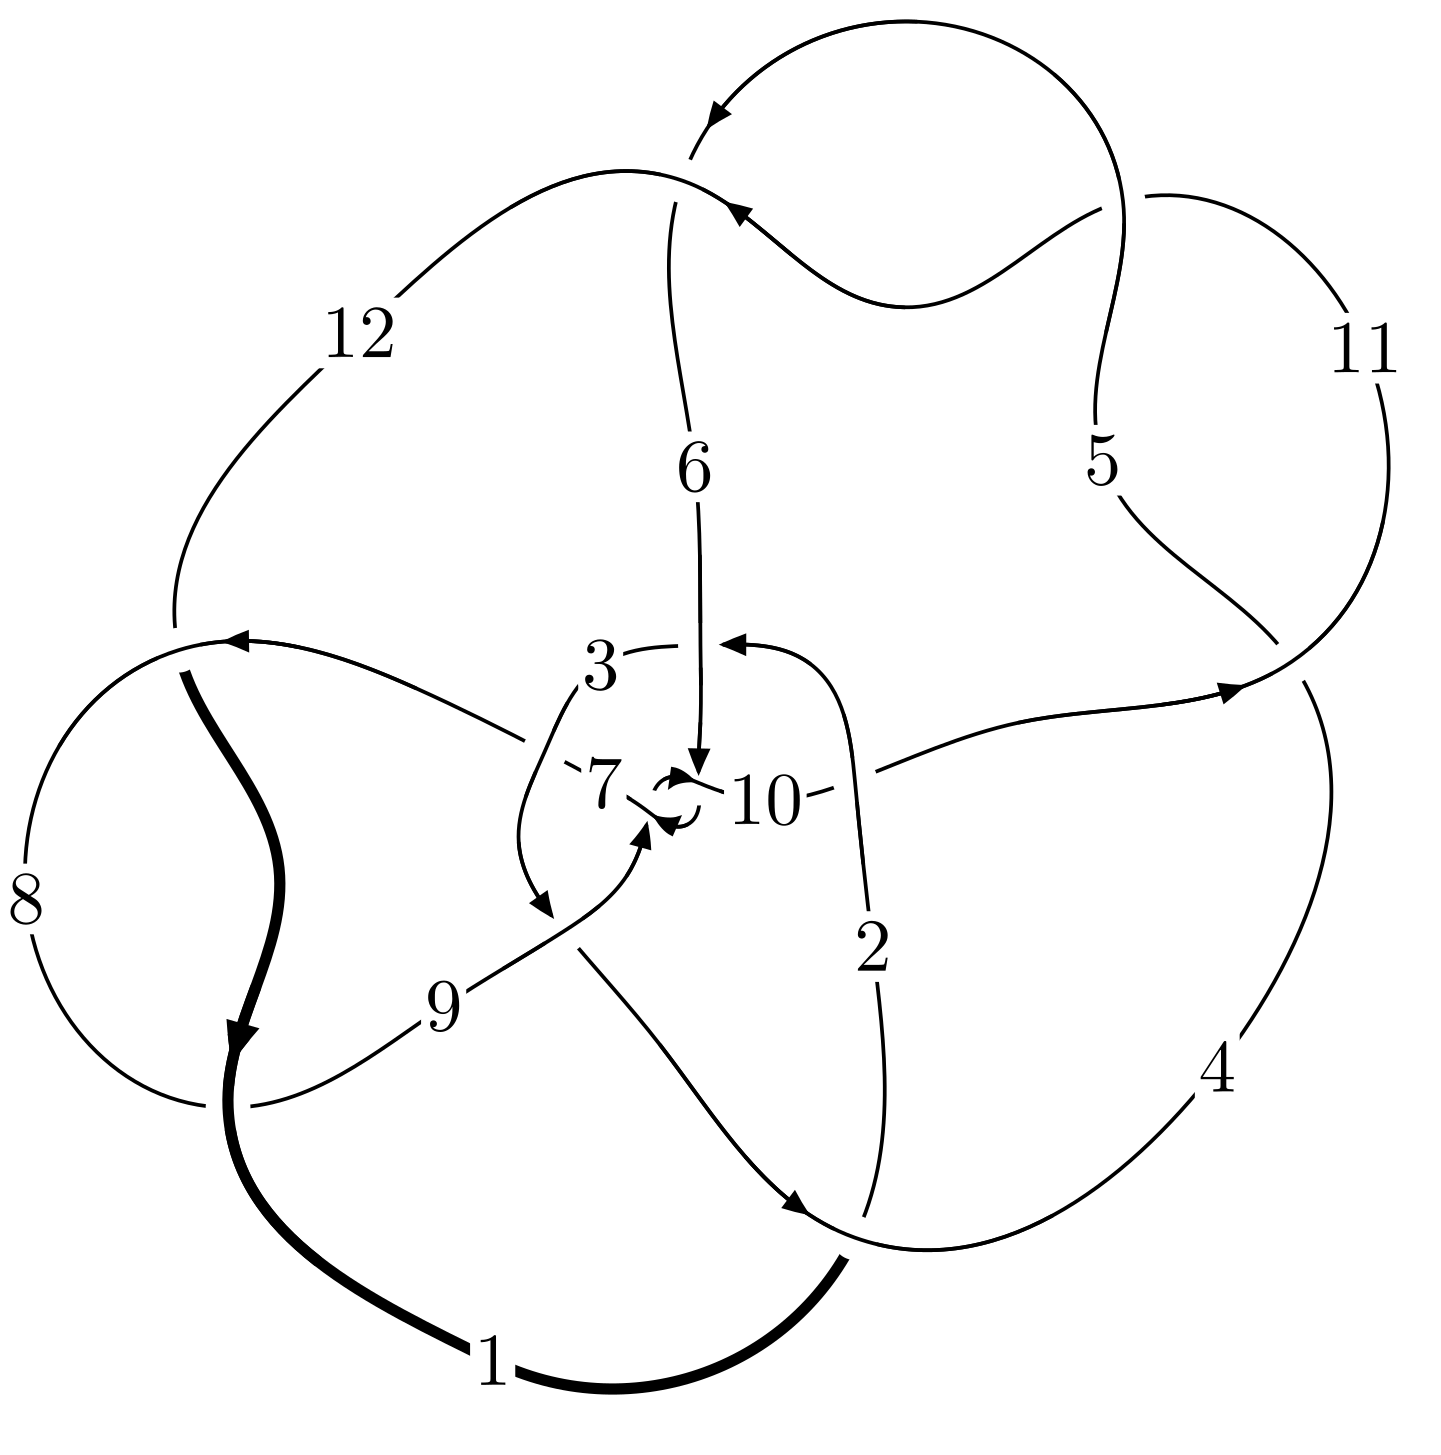
\includegraphics[width=112pt]{../../../GIT/diagram.site/Diagrams/png/1730_12a_0929.png}\\
\ \ \ A knot diagram\footnotemark}&
\allowdisplaybreaks
\textbf{Linearized knot diagam} \\
\cline{2-2}
 &
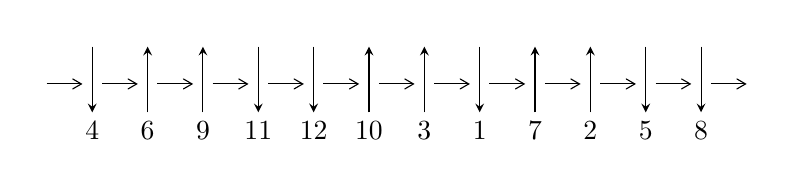
\begin{tikzpicture}[x=20pt, y=17pt]
	% nodes
	\node (C0) at (0, 0) {};
	\node (C1) at (1, 0) {};
	\node (C1U) at (1, +1) {};
	\node (C1D) at (1, -1) {4};

	\node (C2) at (2, 0) {};
	\node (C2U) at (2, +1) {};
	\node (C2D) at (2, -1) {6};

	\node (C3) at (3, 0) {};
	\node (C3U) at (3, +1) {};
	\node (C3D) at (3, -1) {9};

	\node (C4) at (4, 0) {};
	\node (C4U) at (4, +1) {};
	\node (C4D) at (4, -1) {11};

	\node (C5) at (5, 0) {};
	\node (C5U) at (5, +1) {};
	\node (C5D) at (5, -1) {12};

	\node (C6) at (6, 0) {};
	\node (C6U) at (6, +1) {};
	\node (C6D) at (6, -1) {10};

	\node (C7) at (7, 0) {};
	\node (C7U) at (7, +1) {};
	\node (C7D) at (7, -1) {3};

	\node (C8) at (8, 0) {};
	\node (C8U) at (8, +1) {};
	\node (C8D) at (8, -1) {1};

	\node (C9) at (9, 0) {};
	\node (C9U) at (9, +1) {};
	\node (C9D) at (9, -1) {7};

	\node (C10) at (10, 0) {};
	\node (C10U) at (10, +1) {};
	\node (C10D) at (10, -1) {2};

	\node (C11) at (11, 0) {};
	\node (C11U) at (11, +1) {};
	\node (C11D) at (11, -1) {5};

	\node (C12) at (12, 0) {};
	\node (C12U) at (12, +1) {};
	\node (C12D) at (12, -1) {8};
	\node (C13) at (13, 0) {};

	% arrows
	\draw[->,>={angle 60}]
	(C0) edge (C1) (C1) edge (C2) (C2) edge (C3) (C3) edge (C4) (C4) edge (C5) (C5) edge (C6) (C6) edge (C7) (C7) edge (C8) (C8) edge (C9) (C9) edge (C10) (C10) edge (C11) (C11) edge (C12) (C12) edge (C13) ;	\draw[->,>=stealth]
	(C1U) edge (C1D) (C2D) edge (C2U) (C3D) edge (C3U) (C4U) edge (C4D) (C5U) edge (C5D) (C6D) edge (C6U) (C7D) edge (C7U) (C8U) edge (C8D) (C9D) edge (C9U) (C10D) edge (C10U) (C11U) edge (C11D) (C12U) edge (C12D) ;
	\end{tikzpicture} \\
\hhline{~~} \\& 
\textbf{Solving Sequence} \\ \cline{2-2} 
 &
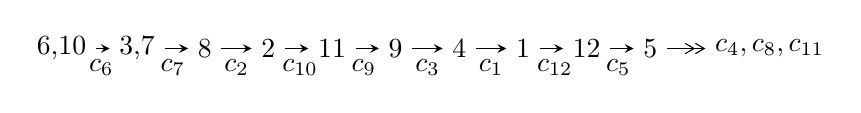
\begin{tikzpicture}[x=23pt, y=7pt]
	% node
	\node (A0) at (-1/8, 0) {6,10};
	\node (A1) at (17/16, 0) {3,7};
	\node (A2) at (17/8, 0) {8};
	\node (A3) at (25/8, 0) {2};
	\node (A4) at (33/8, 0) {11};
	\node (A5) at (41/8, 0) {9};
	\node (A6) at (49/8, 0) {4};
	\node (A7) at (57/8, 0) {1};
	\node (A8) at (65/8, 0) {12};
	\node (A9) at (73/8, 0) {5};
	\node (C1) at (1/2, -1) {$c_{6}$};
	\node (C2) at (13/8, -1) {$c_{7}$};
	\node (C3) at (21/8, -1) {$c_{2}$};
	\node (C4) at (29/8, -1) {$c_{10}$};
	\node (C5) at (37/8, -1) {$c_{9}$};
	\node (C6) at (45/8, -1) {$c_{3}$};
	\node (C7) at (53/8, -1) {$c_{1}$};
	\node (C8) at (61/8, -1) {$c_{12}$};
	\node (C9) at (69/8, -1) {$c_{5}$};
	\node (A10) at (11, 0) {$c_{4},c_{8},c_{11}$};

	% edge
	\draw[->,>=stealth]	
	(A0) edge (A1) (A1) edge (A2) (A2) edge (A3) (A3) edge (A4) (A4) edge (A5) (A5) edge (A6) (A6) edge (A7) (A7) edge (A8) (A8) edge (A9) ;
	\draw[->>,>={angle 60}]	
	(A9) edge (A10);
\end{tikzpicture} \\ 

\end{tabular} \\

\footnotetext{
The image of knot diagram is generated by the software ``\textbf{Draw programme}" developed by Andrew Bartholomew(\url{http://www.layer8.co.uk/maths/draw/index.htm\#Running-draw}), where we modified some parts for our purpose(\url{https://github.com/CATsTAILs/LinksPainter}).
}\phantom \\ \newline 
\centering \textbf{Ideals for irreducible components\footnotemark of $X_{\text{par}}$} 
 
\begin{align*}
I^u_{1}&=\langle 
7.70151\times10^{505} u^{138}-3.75072\times10^{506} u^{137}+\cdots+1.06895\times10^{506} b-8.54489\times10^{505},\\
\phantom{I^u_{1}}&\phantom{= \langle  }-1.85390\times10^{506} u^{138}+8.48171\times10^{506} u^{137}+\cdots+1.06895\times10^{506} a-1.47936\times10^{507},\\
\phantom{I^u_{1}}&\phantom{= \langle  }u^{139}-5 u^{138}+\cdots-5 u-1\rangle \\
I^u_{2}&=\langle 
-74739457095708 u^{37}-838683780419238 u^{36}+\cdots+399763050242851 b-1278150090688057,\\
\phantom{I^u_{2}}&\phantom{= \langle  }716983712604222 u^{37}+3614680862920783 u^{36}+\cdots+399763050242851 a+442429692628259,\\
\phantom{I^u_{2}}&\phantom{= \langle  }u^{38}+6 u^{37}+\cdots+8 u+1\rangle \\
\\
\end{align*}
\raggedright * 2 irreducible components of $\dim_{\mathbb{C}}=0$, with total 177 representations.\\
\footnotetext{All coefficients of polynomials are rational numbers. But the coefficients are sometimes approximated in decimal forms when there is not enough margin.}
\newpage
\renewcommand{\arraystretch}{1}
\centering \section*{I. $I^u_{1}= \langle 7.70\times10^{505} u^{138}-3.75\times10^{506} u^{137}+\cdots+1.07\times10^{506} b-8.54\times10^{505},\;-1.85\times10^{506} u^{138}+8.48\times10^{506} u^{137}+\cdots+1.07\times10^{506} a-1.48\times10^{507},\;u^{139}-5 u^{138}+\cdots-5 u-1 \rangle$}
\flushleft \textbf{(i) Arc colorings}\\
\begin{tabular}{m{7pt} m{180pt} m{7pt} m{180pt} }
\flushright $a_{6}=$&$\begin{pmatrix}1\\0\end{pmatrix}$ \\
\flushright $a_{10}=$&$\begin{pmatrix}0\\u\end{pmatrix}$ \\
\flushright $a_{3}=$&$\begin{pmatrix}1.73432 u^{138}-7.93462 u^{137}+\cdots+278.883 u+13.8394\\-0.720474 u^{138}+3.50880 u^{137}+\cdots-10.8066 u+0.799373\end{pmatrix}$ \\
\flushright $a_{7}=$&$\begin{pmatrix}1\\- u^2\end{pmatrix}$ \\
\flushright $a_{8}=$&$\begin{pmatrix}0.735856 u^{138}-4.21108 u^{137}+\cdots+235.088 u-15.1454\\-0.0760587 u^{138}-0.0133702 u^{137}+\cdots+7.60471 u+1.60285\end{pmatrix}$ \\
\flushright $a_{2}=$&$\begin{pmatrix}2.45479 u^{138}-11.4434 u^{137}+\cdots+289.689 u+13.0400\\-0.720474 u^{138}+3.50880 u^{137}+\cdots-10.8066 u+0.799373\end{pmatrix}$ \\
\flushright $a_{11}=$&$\begin{pmatrix}1.23653 u^{138}-6.01119 u^{137}+\cdots-415.957 u+18.7604\\0.0609717 u^{138}-0.629528 u^{137}+\cdots+14.1572 u-0.658718\end{pmatrix}$ \\
\flushright $a_{9}=$&$\begin{pmatrix}- u\\u^3+u\end{pmatrix}$ \\
\flushright $a_{4}=$&$\begin{pmatrix}2.46548 u^{138}-11.2941 u^{137}+\cdots+280.398 u+13.8012\\-0.485275 u^{138}+2.47123 u^{137}+\cdots-14.5343 u+0.541178\end{pmatrix}$ \\
\flushright $a_{1}=$&$\begin{pmatrix}2.38158 u^{138}-11.6726 u^{137}+\cdots-27.2525 u-18.2120\\-1.21154 u^{138}+6.00159 u^{137}+\cdots-19.9200 u-2.25614\end{pmatrix}$ \\
\flushright $a_{12}=$&$\begin{pmatrix}-0.0581799 u^{138}-0.510923 u^{137}+\cdots-265.552 u+14.6717\\-0.782724 u^{138}+3.73557 u^{137}+\cdots+0.462355 u-2.95331\end{pmatrix}$ \\
\flushright $a_{5}=$&$\begin{pmatrix}0.801704 u^{138}-2.88019 u^{137}+\cdots-374.674 u+30.2259\\-0.0114680 u^{138}+0.203173 u^{137}+\cdots+18.2793 u-0.985923\end{pmatrix}$\\&\end{tabular}
\flushleft \textbf{(ii) Obstruction class $= -1$}\\~\\
\flushleft \textbf{(iii) Cusp Shapes $= -2.93883 u^{138}+13.5235 u^{137}+\cdots-86.5187 u-10.5376$}\\~\\
\newpage\renewcommand{\arraystretch}{1}
\flushleft \textbf{(iv) u-Polynomials at the component}\newline \\
\begin{tabular}{m{50pt}|m{274pt}}
Crossings & \hspace{64pt}u-Polynomials at each crossing \\
\hline $$\begin{aligned}c_{1}\end{aligned}$$&$\begin{aligned}
&u^{139}+12 u^{138}+\cdots-96031942 u-12031189
\end{aligned}$\\
\hline $$\begin{aligned}c_{2}\end{aligned}$$&$\begin{aligned}
&u^{139}+20 u^{137}+\cdots-139979106 u-14998159
\end{aligned}$\\
\hline $$\begin{aligned}c_{3}\end{aligned}$$&$\begin{aligned}
&u^{139}- u^{138}+\cdots-67319757 u-11261219
\end{aligned}$\\
\hline $$\begin{aligned}c_{4},c_{5},c_{11}\end{aligned}$$&$\begin{aligned}
&u^{139}- u^{138}+\cdots-45 u+1
\end{aligned}$\\
\hline $$\begin{aligned}c_{6},c_{9}\end{aligned}$$&$\begin{aligned}
&u^{139}+5 u^{138}+\cdots-5 u+1
\end{aligned}$\\
\hline $$\begin{aligned}c_{7}\end{aligned}$$&$\begin{aligned}
&u^{139}- u^{138}+\cdots-1730911 u-412087
\end{aligned}$\\
\hline $$\begin{aligned}c_{8},c_{12}\end{aligned}$$&$\begin{aligned}
&u^{139}- u^{138}+\cdots+1535 u+59
\end{aligned}$\\
\hline $$\begin{aligned}c_{10}\end{aligned}$$&$\begin{aligned}
&u^{139}-6 u^{138}+\cdots-7021256335 u-1610458073
\end{aligned}$\\
\hline
\end{tabular}\\~\\
\newpage\renewcommand{\arraystretch}{1}
\flushleft \textbf{(v) Riley Polynomials at the component}\newline \\
\begin{tabular}{m{50pt}|m{274pt}}
Crossings & \hspace{64pt}Riley Polynomials at each crossing \\
\hline $$\begin{aligned}c_{1}\end{aligned}$$&$\begin{aligned}
&y^{139}-68 y^{138}+\cdots-3265430574626558 y-144749508753721
\end{aligned}$\\
\hline $$\begin{aligned}c_{2}\end{aligned}$$&$\begin{aligned}
&y^{139}+40 y^{138}+\cdots-6420905976964404 y-224944773389281
\end{aligned}$\\
\hline $$\begin{aligned}c_{3}\end{aligned}$$&$\begin{aligned}
&y^{139}+51 y^{138}+\cdots-3672999278065189 y-126815053365961
\end{aligned}$\\
\hline $$\begin{aligned}c_{4},c_{5},c_{11}\end{aligned}$$&$\begin{aligned}
&y^{139}-139 y^{138}+\cdots+167 y-1
\end{aligned}$\\
\hline $$\begin{aligned}c_{6},c_{9}\end{aligned}$$&$\begin{aligned}
&y^{139}+101 y^{138}+\cdots+71 y-1
\end{aligned}$\\
\hline $$\begin{aligned}c_{7}\end{aligned}$$&$\begin{aligned}
&y^{139}+35 y^{138}+\cdots-4614590704711 y-169815695569
\end{aligned}$\\
\hline $$\begin{aligned}c_{8},c_{12}\end{aligned}$$&$\begin{aligned}
&y^{139}-85 y^{138}+\cdots+3775647 y-3481
\end{aligned}$\\
\hline $$\begin{aligned}c_{10}\end{aligned}$$&$\begin{aligned}
&y^{139}+58 y^{138}+\cdots-8.30\times10^{19} y-2.59\times10^{18}
\end{aligned}$\\
\hline
\end{tabular}\\~\\
\newpage\flushleft \textbf{(vi) Complex Volumes and Cusp Shapes}
$$\begin{array}{c|c|c}  
\text{Solutions to }I^u_{1}& \I (\text{vol} + \sqrt{-1}CS) & \text{Cusp shape}\\
 \hline 
\begin{aligned}
u &= -0.632104 + 0.764385 I \\
a &= -1.064890 - 0.857259 I \\
b &= \phantom{-}0.930191 + 0.078128 I\end{aligned}
 & -3.62053 - 2.47278 I & \phantom{-0.000000 } 0 \\ \hline\begin{aligned}
u &= -0.632104 - 0.764385 I \\
a &= -1.064890 + 0.857259 I \\
b &= \phantom{-}0.930191 - 0.078128 I\end{aligned}
 & -3.62053 + 2.47278 I & \phantom{-0.000000 } 0 \\ \hline\begin{aligned}
u &= -0.625186 + 0.814814 I \\
a &= \phantom{-}0.805602 + 0.418623 I \\
b &= -0.638835 + 0.193995 I\end{aligned}
 & \phantom{-}0.79095 - 2.44484 I & \phantom{-0.000000 } 0 \\ \hline\begin{aligned}
u &= -0.625186 - 0.814814 I \\
a &= \phantom{-}0.805602 - 0.418623 I \\
b &= -0.638835 - 0.193995 I\end{aligned}
 & \phantom{-}0.79095 + 2.44484 I & \phantom{-0.000000 } 0 \\ \hline\begin{aligned}
u &= -0.578146 + 0.849733 I \\
a &= -1.252290 + 0.061980 I \\
b &= \phantom{-}0.442621 - 0.563800 I\end{aligned}
 & -4.42501 - 3.02023 I & \phantom{-0.000000 } 0 \\ \hline\begin{aligned}
u &= -0.578146 - 0.849733 I \\
a &= -1.252290 - 0.061980 I \\
b &= \phantom{-}0.442621 + 0.563800 I\end{aligned}
 & -4.42501 + 3.02023 I & \phantom{-0.000000 } 0 \\ \hline\begin{aligned}
u &= -0.450126 + 0.939673 I \\
a &= -0.77915 - 1.58367 I \\
b &= \phantom{-}0.12832 - 1.64050 I\end{aligned}
 & -2.51785 - 5.09124 I & \phantom{-0.000000 } 0 \\ \hline\begin{aligned}
u &= -0.450126 - 0.939673 I \\
a &= -0.77915 + 1.58367 I \\
b &= \phantom{-}0.12832 + 1.64050 I\end{aligned}
 & -2.51785 + 5.09124 I & \phantom{-0.000000 } 0 \\ \hline\begin{aligned}
u &= \phantom{-}0.040562 + 0.956173 I \\
a &= \phantom{-}0.80061 - 1.50522 I \\
b &= \phantom{-}0.154062 - 1.006350 I\end{aligned}
 & -1.93236 - 1.50203 I & \phantom{-0.000000 } 0 \\ \hline\begin{aligned}
u &= \phantom{-}0.040562 - 0.956173 I \\
a &= \phantom{-}0.80061 + 1.50522 I \\
b &= \phantom{-}0.154062 + 1.006350 I\end{aligned}
 & -1.93236 + 1.50203 I & \phantom{-0.000000 } 0\\
 \hline 
 \end{array}$$\newpage$$\begin{array}{c|c|c}  
\text{Solutions to }I^u_{1}& \I (\text{vol} + \sqrt{-1}CS) & \text{Cusp shape}\\
 \hline 
\begin{aligned}
u &= -0.376090 + 0.975853 I \\
a &= \phantom{-}0.299159 + 1.227920 I \\
b &= -0.227847 + 0.359081 I\end{aligned}
 & \phantom{-}0.20583 - 2.11439 I & \phantom{-0.000000 } 0 \\ \hline\begin{aligned}
u &= -0.376090 - 0.975853 I \\
a &= \phantom{-}0.299159 - 1.227920 I \\
b &= -0.227847 - 0.359081 I\end{aligned}
 & \phantom{-}0.20583 + 2.11439 I & \phantom{-0.000000 } 0 \\ \hline\begin{aligned}
u &= -0.097694 + 0.948171 I \\
a &= -0.18979 - 1.76123 I \\
b &= -0.538958 - 0.292799 I\end{aligned}
 & -3.78394 - 0.07176 I & \phantom{-0.000000 } 0 \\ \hline\begin{aligned}
u &= -0.097694 - 0.948171 I \\
a &= -0.18979 + 1.76123 I \\
b &= -0.538958 + 0.292799 I\end{aligned}
 & -3.78394 + 0.07176 I & \phantom{-0.000000 } 0 \\ \hline\begin{aligned}
u &= \phantom{-}1.054900 + 0.033506 I \\
a &= -0.350782 + 0.054072 I \\
b &= \phantom{-}0.191210 - 1.182360 I\end{aligned}
 & -11.98150 - 0.43899 I & \phantom{-0.000000 } 0 \\ \hline\begin{aligned}
u &= \phantom{-}1.054900 - 0.033506 I \\
a &= -0.350782 - 0.054072 I \\
b &= \phantom{-}0.191210 + 1.182360 I\end{aligned}
 & -11.98150 + 0.43899 I & \phantom{-0.000000 } 0 \\ \hline\begin{aligned}
u &= \phantom{-}0.200437 + 1.044810 I \\
a &= -0.00787 + 1.78491 I \\
b &= \phantom{-}0.97940 + 1.44776 I\end{aligned}
 & -1.89065 + 2.87565 I & \phantom{-0.000000 } 0 \\ \hline\begin{aligned}
u &= \phantom{-}0.200437 - 1.044810 I \\
a &= -0.00787 - 1.78491 I \\
b &= \phantom{-}0.97940 - 1.44776 I\end{aligned}
 & -1.89065 - 2.87565 I & \phantom{-0.000000 } 0 \\ \hline\begin{aligned}
u &= \phantom{-}0.052430 + 1.085180 I \\
a &= \phantom{-}0.083079 + 0.887851 I \\
b &= \phantom{-}1.34567 + 0.62743 I\end{aligned}
 & -2.17992 + 2.23027 I & \phantom{-0.000000 } 0 \\ \hline\begin{aligned}
u &= \phantom{-}0.052430 - 1.085180 I \\
a &= \phantom{-}0.083079 - 0.887851 I \\
b &= \phantom{-}1.34567 - 0.62743 I\end{aligned}
 & -2.17992 - 2.23027 I & \phantom{-0.000000 } 0\\
 \hline 
 \end{array}$$\newpage$$\begin{array}{c|c|c}  
\text{Solutions to }I^u_{1}& \I (\text{vol} + \sqrt{-1}CS) & \text{Cusp shape}\\
 \hline 
\begin{aligned}
u &= \phantom{-}0.133183 + 1.078660 I \\
a &= \phantom{-}0.269627 + 0.788037 I \\
b &= -1.041810 + 0.142681 I\end{aligned}
 & -6.34074 + 5.65719 I & \phantom{-0.000000 } 0 \\ \hline\begin{aligned}
u &= \phantom{-}0.133183 - 1.078660 I \\
a &= \phantom{-}0.269627 - 0.788037 I \\
b &= -1.041810 - 0.142681 I\end{aligned}
 & -6.34074 - 5.65719 I & \phantom{-0.000000 } 0 \\ \hline\begin{aligned}
u &= -0.884291\phantom{ +0.000000I} \\
a &= \phantom{-}0.135616\phantom{ +0.000000I} \\
b &= \phantom{-}0.828989\phantom{ +0.000000I}\end{aligned}
 & \phantom{-}1.73740\phantom{ +0.000000I} & \phantom{-0.000000 } 0 \\ \hline\begin{aligned}
u &= \phantom{-}1.122850 + 0.143683 I \\
a &= -0.0144874 - 0.0238569 I \\
b &= \phantom{-}0.913772 + 1.019110 I\end{aligned}
 & -9.3265 + 13.2419 I & \phantom{-0.000000 } 0 \\ \hline\begin{aligned}
u &= \phantom{-}1.122850 - 0.143683 I \\
a &= -0.0144874 + 0.0238569 I \\
b &= \phantom{-}0.913772 - 1.019110 I\end{aligned}
 & -9.3265 - 13.2419 I & \phantom{-0.000000 } 0 \\ \hline\begin{aligned}
u &= -0.030369 + 1.141630 I \\
a &= -1.13180 + 1.56529 I \\
b &= -0.827680 + 0.856148 I\end{aligned}
 & -7.14553 - 4.22155 I & \phantom{-0.000000 } 0 \\ \hline\begin{aligned}
u &= -0.030369 - 1.141630 I \\
a &= -1.13180 - 1.56529 I \\
b &= -0.827680 - 0.856148 I\end{aligned}
 & -7.14553 + 4.22155 I & \phantom{-0.000000 } 0 \\ \hline\begin{aligned}
u &= \phantom{-}0.574161 + 0.999656 I \\
a &= -1.038430 + 0.387110 I \\
b &= -0.742550 + 0.859820 I\end{aligned}
 & -4.00102 + 4.85639 I & \phantom{-0.000000 } 0 \\ \hline\begin{aligned}
u &= \phantom{-}0.574161 - 0.999656 I \\
a &= -1.038430 - 0.387110 I \\
b &= -0.742550 - 0.859820 I\end{aligned}
 & -4.00102 - 4.85639 I & \phantom{-0.000000 } 0 \\ \hline\begin{aligned}
u &= \phantom{-}0.376627 + 1.096920 I \\
a &= \phantom{-}0.08063 + 2.21291 I \\
b &= \phantom{-}0.732094 + 0.195650 I\end{aligned}
 & -9.83431 + 8.73999 I & \phantom{-0.000000 } 0\\
 \hline 
 \end{array}$$\newpage$$\begin{array}{c|c|c}  
\text{Solutions to }I^u_{1}& \I (\text{vol} + \sqrt{-1}CS) & \text{Cusp shape}\\
 \hline 
\begin{aligned}
u &= \phantom{-}0.376627 - 1.096920 I \\
a &= \phantom{-}0.08063 - 2.21291 I \\
b &= \phantom{-}0.732094 - 0.195650 I\end{aligned}
 & -9.83431 - 8.73999 I & \phantom{-0.000000 } 0 \\ \hline\begin{aligned}
u &= \phantom{-}0.131427 + 1.154940 I \\
a &= -0.47784 + 1.44960 I \\
b &= -1.14341 + 1.07951 I\end{aligned}
 & -6.18385 + 5.50700 I & \phantom{-0.000000 } 0 \\ \hline\begin{aligned}
u &= \phantom{-}0.131427 - 1.154940 I \\
a &= -0.47784 - 1.44960 I \\
b &= -1.14341 - 1.07951 I\end{aligned}
 & -6.18385 - 5.50700 I & \phantom{-0.000000 } 0 \\ \hline\begin{aligned}
u &= -0.033659 + 1.162790 I \\
a &= -0.154800 - 1.358090 I \\
b &= -0.892725 - 1.067090 I\end{aligned}
 & -3.70268 - 1.30296 I & \phantom{-0.000000 } 0 \\ \hline\begin{aligned}
u &= -0.033659 - 1.162790 I \\
a &= -0.154800 + 1.358090 I \\
b &= -0.892725 + 1.067090 I\end{aligned}
 & -3.70268 + 1.30296 I & \phantom{-0.000000 } 0 \\ \hline\begin{aligned}
u &= \phantom{-}0.293787 + 1.128340 I \\
a &= -0.17563 - 1.98365 I \\
b &= -0.285408 - 0.485364 I\end{aligned}
 & -4.32303 + 6.86710 I & \phantom{-0.000000 } 0 \\ \hline\begin{aligned}
u &= \phantom{-}0.293787 - 1.128340 I \\
a &= -0.17563 + 1.98365 I \\
b &= -0.285408 + 0.485364 I\end{aligned}
 & -4.32303 - 6.86710 I & \phantom{-0.000000 } 0 \\ \hline\begin{aligned}
u &= -0.327936 + 1.120870 I \\
a &= -0.27163 + 2.31639 I \\
b &= -1.41225 + 2.17689 I\end{aligned}
 & -10.47560 - 9.06708 I & \phantom{-0.000000 } 0 \\ \hline\begin{aligned}
u &= -0.327936 - 1.120870 I \\
a &= -0.27163 - 2.31639 I \\
b &= -1.41225 - 2.17689 I\end{aligned}
 & -10.47560 + 9.06708 I & \phantom{-0.000000 } 0 \\ \hline\begin{aligned}
u &= \phantom{-}1.164710 + 0.145738 I \\
a &= -0.0718814 - 0.0205685 I \\
b &= -0.663783 - 0.821663 I\end{aligned}
 & -2.70772 + 8.73976 I & \phantom{-0.000000 } 0\\
 \hline 
 \end{array}$$\newpage$$\begin{array}{c|c|c}  
\text{Solutions to }I^u_{1}& \I (\text{vol} + \sqrt{-1}CS) & \text{Cusp shape}\\
 \hline 
\begin{aligned}
u &= \phantom{-}1.164710 - 0.145738 I \\
a &= -0.0718814 + 0.0205685 I \\
b &= -0.663783 + 0.821663 I\end{aligned}
 & -2.70772 - 8.73976 I & \phantom{-0.000000 } 0 \\ \hline\begin{aligned}
u &= \phantom{-}0.216339 + 1.157270 I \\
a &= -0.11963 - 1.76006 I \\
b &= -1.29983 - 1.46989 I\end{aligned}
 & -7.96668 + 6.49431 I & \phantom{-0.000000 } 0 \\ \hline\begin{aligned}
u &= \phantom{-}0.216339 - 1.157270 I \\
a &= -0.11963 + 1.76006 I \\
b &= -1.29983 + 1.46989 I\end{aligned}
 & -7.96668 - 6.49431 I & \phantom{-0.000000 } 0 \\ \hline\begin{aligned}
u &= -0.603808 + 0.512147 I \\
a &= \phantom{-}1.42525 + 0.13019 I \\
b &= \phantom{-}0.687606 + 1.058580 I\end{aligned}
 & -1.35003 + 0.84890 I & \phantom{-0.000000 } 0 \\ \hline\begin{aligned}
u &= -0.603808 - 0.512147 I \\
a &= \phantom{-}1.42525 - 0.13019 I \\
b &= \phantom{-}0.687606 - 1.058580 I\end{aligned}
 & -1.35003 - 0.84890 I & \phantom{-0.000000 } 0 \\ \hline\begin{aligned}
u &= \phantom{-}1.209830 + 0.053647 I \\
a &= \phantom{-}0.169389 + 0.030182 I \\
b &= \phantom{-}0.254752 + 0.774658 I\end{aligned}
 & -3.55913 + 2.84298 I & \phantom{-0.000000 } 0 \\ \hline\begin{aligned}
u &= \phantom{-}1.209830 - 0.053647 I \\
a &= \phantom{-}0.169389 - 0.030182 I \\
b &= \phantom{-}0.254752 - 0.774658 I\end{aligned}
 & -3.55913 - 2.84298 I & \phantom{-0.000000 } 0 \\ \hline\begin{aligned}
u &= -0.081245 + 1.213710 I \\
a &= \phantom{-}1.20424 + 2.16299 I \\
b &= -0.426972 + 1.087010 I\end{aligned}
 & -13.7202 - 7.3631 I & \phantom{-0.000000 } 0 \\ \hline\begin{aligned}
u &= -0.081245 - 1.213710 I \\
a &= \phantom{-}1.20424 - 2.16299 I \\
b &= -0.426972 - 1.087010 I\end{aligned}
 & -13.7202 + 7.3631 I & \phantom{-0.000000 } 0 \\ \hline\begin{aligned}
u &= -0.779454\phantom{ +0.000000I} \\
a &= \phantom{-}0.0601539\phantom{ +0.000000I} \\
b &= -1.60160\phantom{ +0.000000I}\end{aligned}
 & -2.60324\phantom{ +0.000000I} & \phantom{-0.000000 } 0\\
 \hline 
 \end{array}$$\newpage$$\begin{array}{c|c|c}  
\text{Solutions to }I^u_{1}& \I (\text{vol} + \sqrt{-1}CS) & \text{Cusp shape}\\
 \hline 
\begin{aligned}
u &= -1.147100 + 0.428093 I \\
a &= \phantom{-}0.0746036 + 0.0133176 I \\
b &= -0.548048 + 0.264373 I\end{aligned}
 & \phantom{-}1.64726 - 2.96897 I & \phantom{-0.000000 } 0 \\ \hline\begin{aligned}
u &= -1.147100 - 0.428093 I \\
a &= \phantom{-}0.0746036 - 0.0133176 I \\
b &= -0.548048 - 0.264373 I\end{aligned}
 & \phantom{-}1.64726 + 2.96897 I & \phantom{-0.000000 } 0 \\ \hline\begin{aligned}
u &= -1.221970 + 0.106384 I \\
a &= -0.130642 + 0.070039 I \\
b &= \phantom{-}0.641240 - 0.899596 I\end{aligned}
 & -5.40420 - 6.34999 I & \phantom{-0.000000 } 0 \\ \hline\begin{aligned}
u &= -1.221970 - 0.106384 I \\
a &= -0.130642 - 0.070039 I \\
b &= \phantom{-}0.641240 + 0.899596 I\end{aligned}
 & -5.40420 + 6.34999 I & \phantom{-0.000000 } 0 \\ \hline\begin{aligned}
u &= \phantom{-}0.061866 + 1.229080 I \\
a &= \phantom{-}1.10101 - 2.22020 I \\
b &= \phantom{-}1.69509 - 2.45035 I\end{aligned}
 & -13.9888 + 7.0441 I & \phantom{-0.000000 } 0 \\ \hline\begin{aligned}
u &= \phantom{-}0.061866 - 1.229080 I \\
a &= \phantom{-}1.10101 + 2.22020 I \\
b &= \phantom{-}1.69509 + 2.45035 I\end{aligned}
 & -13.9888 - 7.0441 I & \phantom{-0.000000 } 0 \\ \hline\begin{aligned}
u &= -0.057965 + 1.240160 I \\
a &= -0.68750 - 1.69985 I \\
b &= \phantom{-}0.502615 - 0.896052 I\end{aligned}
 & -7.51703 - 4.43921 I & \phantom{-0.000000 } 0 \\ \hline\begin{aligned}
u &= -0.057965 - 1.240160 I \\
a &= -0.68750 + 1.69985 I \\
b &= \phantom{-}0.502615 + 0.896052 I\end{aligned}
 & -7.51703 + 4.43921 I & \phantom{-0.000000 } 0 \\ \hline\begin{aligned}
u &= \phantom{-}0.693216 + 0.294172 I \\
a &= -1.235230 - 0.606825 I \\
b &= \phantom{-}1.234120 - 0.277966 I\end{aligned}
 & -7.46136 - 4.66764 I & \phantom{-0.000000 } 0 \\ \hline\begin{aligned}
u &= \phantom{-}0.693216 - 0.294172 I \\
a &= -1.235230 + 0.606825 I \\
b &= \phantom{-}1.234120 + 0.277966 I\end{aligned}
 & -7.46136 + 4.66764 I & \phantom{-0.000000 } 0\\
 \hline 
 \end{array}$$\newpage$$\begin{array}{c|c|c}  
\text{Solutions to }I^u_{1}& \I (\text{vol} + \sqrt{-1}CS) & \text{Cusp shape}\\
 \hline 
\begin{aligned}
u &= -0.740925 + 0.039005 I \\
a &= \phantom{-}0.175208 + 0.012937 I \\
b &= \phantom{-}0.894801 + 0.094130 I\end{aligned}
 & \phantom{-}1.79165 + 0.01807 I & \phantom{-0.000000 } 0 \\ \hline\begin{aligned}
u &= -0.740925 - 0.039005 I \\
a &= \phantom{-}0.175208 - 0.012937 I \\
b &= \phantom{-}0.894801 - 0.094130 I\end{aligned}
 & \phantom{-}1.79165 - 0.01807 I & \phantom{-0.000000 } 0 \\ \hline\begin{aligned}
u &= \phantom{-}0.396515 + 0.626820 I \\
a &= \phantom{-}1.61618 + 0.64913 I \\
b &= \phantom{-}1.043350 - 0.351024 I\end{aligned}
 & -0.806683 - 0.430513 I & \phantom{-0.000000 } 0 \\ \hline\begin{aligned}
u &= \phantom{-}0.396515 - 0.626820 I \\
a &= \phantom{-}1.61618 - 0.64913 I \\
b &= \phantom{-}1.043350 + 0.351024 I\end{aligned}
 & -0.806683 + 0.430513 I & \phantom{-0.000000 } 0 \\ \hline\begin{aligned}
u &= -0.488716 + 1.188780 I \\
a &= \phantom{-}0.059634 - 1.120490 I \\
b &= \phantom{-}0.571156 - 0.740029 I\end{aligned}
 & -1.77558 - 4.94866 I & \phantom{-0.000000 } 0 \\ \hline\begin{aligned}
u &= -0.488716 - 1.188780 I \\
a &= \phantom{-}0.059634 + 1.120490 I \\
b &= \phantom{-}0.571156 + 0.740029 I\end{aligned}
 & -1.77558 + 4.94866 I & \phantom{-0.000000 } 0 \\ \hline\begin{aligned}
u &= -0.321103 + 1.251180 I \\
a &= -1.01316 + 1.56690 I \\
b &= -1.39219 + 0.69119 I\end{aligned}
 & -6.46785 - 3.98634 I & \phantom{-0.000000 } 0 \\ \hline\begin{aligned}
u &= -0.321103 - 1.251180 I \\
a &= -1.01316 - 1.56690 I \\
b &= -1.39219 - 0.69119 I\end{aligned}
 & -6.46785 + 3.98634 I & \phantom{-0.000000 } 0 \\ \hline\begin{aligned}
u &= -0.023033 + 1.294480 I \\
a &= \phantom{-}0.429469 + 1.221800 I \\
b &= \phantom{-}1.16918 + 1.40255 I\end{aligned}
 & -10.15290 - 2.95176 I & \phantom{-0.000000 } 0 \\ \hline\begin{aligned}
u &= -0.023033 - 1.294480 I \\
a &= \phantom{-}0.429469 - 1.221800 I \\
b &= \phantom{-}1.16918 - 1.40255 I\end{aligned}
 & -10.15290 + 2.95176 I & \phantom{-0.000000 } 0\\
 \hline 
 \end{array}$$\newpage$$\begin{array}{c|c|c}  
\text{Solutions to }I^u_{1}& \I (\text{vol} + \sqrt{-1}CS) & \text{Cusp shape}\\
 \hline 
\begin{aligned}
u &= \phantom{-}0.663270 + 0.227218 I \\
a &= \phantom{-}0.517789 - 0.387904 I \\
b &= -0.698127 - 0.542906 I\end{aligned}
 & -2.15270 - 0.29643 I & \phantom{-0.000000 } 0 \\ \hline\begin{aligned}
u &= \phantom{-}0.663270 - 0.227218 I \\
a &= \phantom{-}0.517789 + 0.387904 I \\
b &= -0.698127 + 0.542906 I\end{aligned}
 & -2.15270 + 0.29643 I & \phantom{-0.000000 } 0 \\ \hline\begin{aligned}
u &= \phantom{-}0.269302 + 1.275940 I \\
a &= \phantom{-}0.23313 + 2.04139 I \\
b &= \phantom{-}0.85140 + 1.32317 I\end{aligned}
 & -3.56123 + 6.01556 I & \phantom{-0.000000 } 0 \\ \hline\begin{aligned}
u &= \phantom{-}0.269302 - 1.275940 I \\
a &= \phantom{-}0.23313 - 2.04139 I \\
b &= \phantom{-}0.85140 - 1.32317 I\end{aligned}
 & -3.56123 - 6.01556 I & \phantom{-0.000000 } 0 \\ \hline\begin{aligned}
u &= \phantom{-}0.231566 + 1.285870 I \\
a &= -0.15984 - 2.29698 I \\
b &= -0.84573 - 1.87240 I\end{aligned}
 & -8.17289 + 8.32891 I & \phantom{-0.000000 } 0 \\ \hline\begin{aligned}
u &= \phantom{-}0.231566 - 1.285870 I \\
a &= -0.15984 + 2.29698 I \\
b &= -0.84573 + 1.87240 I\end{aligned}
 & -8.17289 - 8.32891 I & \phantom{-0.000000 } 0 \\ \hline\begin{aligned}
u &= \phantom{-}0.081050 + 1.310830 I \\
a &= -0.697772 + 0.506852 I \\
b &= -1.39957 + 0.43759 I\end{aligned}
 & -6.71126 - 1.59464 I & \phantom{-0.000000 } 0 \\ \hline\begin{aligned}
u &= \phantom{-}0.081050 - 1.310830 I \\
a &= -0.697772 - 0.506852 I \\
b &= -1.39957 - 0.43759 I\end{aligned}
 & -6.71126 + 1.59464 I & \phantom{-0.000000 } 0 \\ \hline\begin{aligned}
u &= -0.640989 + 0.226911 I \\
a &= -1.19954 + 0.95018 I \\
b &= -1.02641 - 1.01692 I\end{aligned}
 & -7.85912 + 5.38264 I & \phantom{-0.000000 } 0 \\ \hline\begin{aligned}
u &= -0.640989 - 0.226911 I \\
a &= -1.19954 - 0.95018 I \\
b &= -1.02641 + 1.01692 I\end{aligned}
 & -7.85912 - 5.38264 I & \phantom{-0.000000 } 0\\
 \hline 
 \end{array}$$\newpage$$\begin{array}{c|c|c}  
\text{Solutions to }I^u_{1}& \I (\text{vol} + \sqrt{-1}CS) & \text{Cusp shape}\\
 \hline 
\begin{aligned}
u &= -0.066545 + 1.321360 I \\
a &= \phantom{-}0.768645 + 0.747733 I \\
b &= -0.297793 + 0.514659 I\end{aligned}
 & -7.17179 - 0.71597 I & \phantom{-0.000000 } 0 \\ \hline\begin{aligned}
u &= -0.066545 - 1.321360 I \\
a &= \phantom{-}0.768645 - 0.747733 I \\
b &= -0.297793 - 0.514659 I\end{aligned}
 & -7.17179 + 0.71597 I & \phantom{-0.000000 } 0 \\ \hline\begin{aligned}
u &= -0.315227 + 1.288070 I \\
a &= \phantom{-}0.52410 - 1.58607 I \\
b &= \phantom{-}1.01407 - 1.14665 I\end{aligned}
 & -2.20214 - 3.80235 I & \phantom{-0.000000 } 0 \\ \hline\begin{aligned}
u &= -0.315227 - 1.288070 I \\
a &= \phantom{-}0.52410 + 1.58607 I \\
b &= \phantom{-}1.01407 + 1.14665 I\end{aligned}
 & -2.20214 + 3.80235 I & \phantom{-0.000000 } 0 \\ \hline\begin{aligned}
u &= -0.151574 + 1.324020 I \\
a &= -1.34391 - 0.47917 I \\
b &= -0.063819 - 0.637227 I\end{aligned}
 & -12.81730 + 2.75952 I & \phantom{-0.000000 } 0 \\ \hline\begin{aligned}
u &= -0.151574 - 1.324020 I \\
a &= -1.34391 + 0.47917 I \\
b &= -0.063819 + 0.637227 I\end{aligned}
 & -12.81730 - 2.75952 I & \phantom{-0.000000 } 0 \\ \hline\begin{aligned}
u &= -0.291169 + 1.312350 I \\
a &= -0.28843 + 1.95616 I \\
b &= -0.97209 + 1.82682 I\end{aligned}
 & -7.62419 - 4.26111 I & \phantom{-0.000000 } 0 \\ \hline\begin{aligned}
u &= -0.291169 - 1.312350 I \\
a &= -0.28843 - 1.95616 I \\
b &= -0.97209 - 1.82682 I\end{aligned}
 & -7.62419 + 4.26111 I & \phantom{-0.000000 } 0 \\ \hline\begin{aligned}
u &= \phantom{-}0.064319 + 1.349230 I \\
a &= -0.132807 + 0.304254 I \\
b &= \phantom{-}0.766753 + 0.551467 I\end{aligned}
 & -10.16590 - 2.53861 I & \phantom{-0.000000 } 0 \\ \hline\begin{aligned}
u &= \phantom{-}0.064319 - 1.349230 I \\
a &= -0.132807 - 0.304254 I \\
b &= \phantom{-}0.766753 - 0.551467 I\end{aligned}
 & -10.16590 + 2.53861 I & \phantom{-0.000000 } 0\\
 \hline 
 \end{array}$$\newpage$$\begin{array}{c|c|c}  
\text{Solutions to }I^u_{1}& \I (\text{vol} + \sqrt{-1}CS) & \text{Cusp shape}\\
 \hline 
\begin{aligned}
u &= \phantom{-}0.141759 + 1.348390 I \\
a &= \phantom{-}1.280460 - 0.496264 I \\
b &= \phantom{-}2.04695 - 0.81471 I\end{aligned}
 & -12.83850 - 1.98284 I & \phantom{-0.000000 } 0 \\ \hline\begin{aligned}
u &= \phantom{-}0.141759 - 1.348390 I \\
a &= \phantom{-}1.280460 + 0.496264 I \\
b &= \phantom{-}2.04695 + 0.81471 I\end{aligned}
 & -12.83850 + 1.98284 I & \phantom{-0.000000 } 0 \\ \hline\begin{aligned}
u &= \phantom{-}0.312822 + 1.329800 I \\
a &= -0.35508 - 1.68811 I \\
b &= -1.04846 - 0.95234 I\end{aligned}
 & -6.85262 + 3.32305 I & \phantom{-0.000000 } 0 \\ \hline\begin{aligned}
u &= \phantom{-}0.312822 - 1.329800 I \\
a &= -0.35508 + 1.68811 I \\
b &= -1.04846 + 0.95234 I\end{aligned}
 & -6.85262 - 3.32305 I & \phantom{-0.000000 } 0 \\ \hline\begin{aligned}
u &= \phantom{-}0.564982 + 0.246712 I \\
a &= \phantom{-}0.941868 + 0.988039 I \\
b &= -0.778969 + 0.273927 I\end{aligned}
 & -1.74419 - 3.51926 I & \phantom{-0.000000 -}0. + 6.81358 I \\ \hline\begin{aligned}
u &= \phantom{-}0.564982 - 0.246712 I \\
a &= \phantom{-}0.941868 - 0.988039 I \\
b &= -0.778969 - 0.273927 I\end{aligned}
 & -1.74419 + 3.51926 I & \phantom{-0.000000 } 0. - 6.81358 I \\ \hline\begin{aligned}
u &= -0.579514 + 0.172524 I \\
a &= -0.599116 - 0.441227 I \\
b &= -0.651970 + 0.762314 I\end{aligned}
 & -3.10725 - 0.93221 I & -1.69865 + 1.91084 I \\ \hline\begin{aligned}
u &= -0.579514 - 0.172524 I \\
a &= -0.599116 + 0.441227 I \\
b &= -0.651970 - 0.762314 I\end{aligned}
 & -3.10725 + 0.93221 I & -1.69865 - 1.91084 I \\ \hline\begin{aligned}
u &= \phantom{-}0.375731 + 0.430586 I \\
a &= -1.46280 - 1.70331 I \\
b &= \phantom{-}0.121273 + 0.381635 I\end{aligned}
 & -4.73205 - 3.56692 I & -3.56257 + 0.82297 I \\ \hline\begin{aligned}
u &= \phantom{-}0.375731 - 0.430586 I \\
a &= -1.46280 + 1.70331 I \\
b &= \phantom{-}0.121273 - 0.381635 I\end{aligned}
 & -4.73205 + 3.56692 I & -3.56257 - 0.82297 I\\
 \hline 
 \end{array}$$\newpage$$\begin{array}{c|c|c}  
\text{Solutions to }I^u_{1}& \I (\text{vol} + \sqrt{-1}CS) & \text{Cusp shape}\\
 \hline 
\begin{aligned}
u &= \phantom{-}0.551351 + 0.041466 I \\
a &= -0.348797 + 0.159864 I \\
b &= \phantom{-}0.909573 + 0.742731 I\end{aligned}
 & \phantom{-}0.49466 + 2.87994 I & \phantom{-}3.76408 - 7.17730 I \\ \hline\begin{aligned}
u &= \phantom{-}0.551351 - 0.041466 I \\
a &= -0.348797 - 0.159864 I \\
b &= \phantom{-}0.909573 - 0.742731 I\end{aligned}
 & \phantom{-}0.49466 - 2.87994 I & \phantom{-}3.76408 + 7.17730 I \\ \hline\begin{aligned}
u &= \phantom{-}0.50487 + 1.35872 I \\
a &= \phantom{-}0.57340 - 1.32710 I \\
b &= -0.19555 - 1.69780 I\end{aligned}
 & -16.3446 + 5.0785 I & \phantom{-0.000000 } 0 \\ \hline\begin{aligned}
u &= \phantom{-}0.50487 - 1.35872 I \\
a &= \phantom{-}0.57340 + 1.32710 I \\
b &= -0.19555 + 1.69780 I\end{aligned}
 & -16.3446 - 5.0785 I & \phantom{-0.000000 } 0 \\ \hline\begin{aligned}
u &= \phantom{-}0.53916 + 1.35125 I \\
a &= -0.592181 + 1.256510 I \\
b &= \phantom{-}0.77271 + 1.21631 I\end{aligned}
 & -16.0866 + 6.1383 I & \phantom{-0.000000 } 0 \\ \hline\begin{aligned}
u &= \phantom{-}0.53916 - 1.35125 I \\
a &= -0.592181 - 1.256510 I \\
b &= \phantom{-}0.77271 - 1.21631 I\end{aligned}
 & -16.0866 - 6.1383 I & \phantom{-0.000000 } 0 \\ \hline\begin{aligned}
u &= \phantom{-}0.494920 + 0.064945 I \\
a &= -0.201421 + 0.138589 I \\
b &= -0.846145 - 1.054990 I\end{aligned}
 & -4.00307 + 5.55437 I & -0.20630 - 9.80295 I \\ \hline\begin{aligned}
u &= \phantom{-}0.494920 - 0.064945 I \\
a &= -0.201421 - 0.138589 I \\
b &= -0.846145 + 1.054990 I\end{aligned}
 & -4.00307 - 5.55437 I & -0.20630 + 9.80295 I \\ \hline\begin{aligned}
u &= \phantom{-}0.49609 + 1.41761 I \\
a &= \phantom{-}0.06162 + 1.67711 I \\
b &= \phantom{-}1.25880 + 1.44695 I\end{aligned}
 & -14.2338 + 18.9321 I & \phantom{-0.000000 } 0 \\ \hline\begin{aligned}
u &= \phantom{-}0.49609 - 1.41761 I \\
a &= \phantom{-}0.06162 - 1.67711 I \\
b &= \phantom{-}1.25880 - 1.44695 I\end{aligned}
 & -14.2338 - 18.9321 I & \phantom{-0.000000 } 0\\
 \hline 
 \end{array}$$\newpage$$\begin{array}{c|c|c}  
\text{Solutions to }I^u_{1}& \I (\text{vol} + \sqrt{-1}CS) & \text{Cusp shape}\\
 \hline 
\begin{aligned}
u &= \phantom{-}0.52629 + 1.40859 I \\
a &= -0.175667 + 1.314370 I \\
b &= \phantom{-}0.64333 + 1.33059 I\end{aligned}
 & -8.23137 + 8.85985 I & \phantom{-0.000000 } 0 \\ \hline\begin{aligned}
u &= \phantom{-}0.52629 - 1.40859 I \\
a &= -0.175667 - 1.314370 I \\
b &= \phantom{-}0.64333 - 1.33059 I\end{aligned}
 & -8.23137 - 8.85985 I & \phantom{-0.000000 } 0 \\ \hline\begin{aligned}
u &= \phantom{-}0.50533 + 1.42053 I \\
a &= -0.00810 - 1.49369 I \\
b &= -1.00508 - 1.32890 I\end{aligned}
 & -7.6298 + 14.5593 I & \phantom{-0.000000 } 0 \\ \hline\begin{aligned}
u &= \phantom{-}0.50533 - 1.42053 I \\
a &= -0.00810 + 1.49369 I \\
b &= -1.00508 + 1.32890 I\end{aligned}
 & -7.6298 - 14.5593 I & \phantom{-0.000000 } 0 \\ \hline\begin{aligned}
u &= -0.49851 + 1.42956 I \\
a &= -0.042542 + 1.227700 I \\
b &= -0.97671 + 1.06557 I\end{aligned}
 & -3.66903 - 8.81792 I & \phantom{-0.000000 } 0 \\ \hline\begin{aligned}
u &= -0.49851 - 1.42956 I \\
a &= -0.042542 - 1.227700 I \\
b &= -0.97671 - 1.06557 I\end{aligned}
 & -3.66903 + 8.81792 I & \phantom{-0.000000 } 0 \\ \hline\begin{aligned}
u &= -0.52229 + 1.42436 I \\
a &= -0.067096 - 1.388590 I \\
b &= \phantom{-}1.14001 - 1.26236 I\end{aligned}
 & -10.2609 - 12.3841 I & \phantom{-0.000000 } 0 \\ \hline\begin{aligned}
u &= -0.52229 - 1.42436 I \\
a &= -0.067096 + 1.388590 I \\
b &= \phantom{-}1.14001 + 1.26236 I\end{aligned}
 & -10.2609 + 12.3841 I & \phantom{-0.000000 } 0 \\ \hline\begin{aligned}
u &= \phantom{-}0.425096 + 0.199889 I \\
a &= -0.59446 - 1.85856 I \\
b &= -0.496624 + 0.741934 I\end{aligned}
 & -5.16865 - 3.96189 I & -8.75976 - 1.52352 I \\ \hline\begin{aligned}
u &= \phantom{-}0.425096 - 0.199889 I \\
a &= -0.59446 + 1.85856 I \\
b &= -0.496624 - 0.741934 I\end{aligned}
 & -5.16865 + 3.96189 I & -8.75976 + 1.52352 I\\
 \hline 
 \end{array}$$\newpage$$\begin{array}{c|c|c}  
\text{Solutions to }I^u_{1}& \I (\text{vol} + \sqrt{-1}CS) & \text{Cusp shape}\\
 \hline 
\begin{aligned}
u &= \phantom{-}0.49284 + 1.45025 I \\
a &= \phantom{-}0.210900 - 0.948046 I \\
b &= -0.611507 - 0.865321 I\end{aligned}
 & -8.34973 + 3.47434 I & \phantom{-0.000000 } 0 \\ \hline\begin{aligned}
u &= \phantom{-}0.49284 - 1.45025 I \\
a &= \phantom{-}0.210900 + 0.948046 I \\
b &= -0.611507 + 0.865321 I\end{aligned}
 & -8.34973 - 3.47434 I & \phantom{-0.000000 } 0 \\ \hline\begin{aligned}
u &= -0.45669 + 1.46870 I \\
a &= \phantom{-}0.092018 - 0.950393 I \\
b &= \phantom{-}0.698719 - 0.926621 I\end{aligned}
 & -3.66154 - 4.15808 I & \phantom{-0.000000 } 0 \\ \hline\begin{aligned}
u &= -0.45669 - 1.46870 I \\
a &= \phantom{-}0.092018 + 0.950393 I \\
b &= \phantom{-}0.698719 + 0.926621 I\end{aligned}
 & -3.66154 + 4.15808 I & \phantom{-0.000000 } 0 \\ \hline\begin{aligned}
u &= -1.48715 + 0.40226 I \\
a &= \phantom{-}0.0364771 + 0.0056350 I \\
b &= -0.297858 + 0.327164 I\end{aligned}
 & \phantom{-}1.67745 - 2.92146 I & \phantom{-0.000000 } 0 \\ \hline\begin{aligned}
u &= -1.48715 - 0.40226 I \\
a &= \phantom{-}0.0364771 - 0.0056350 I \\
b &= -0.297858 - 0.327164 I\end{aligned}
 & \phantom{-}1.67745 + 2.92146 I & \phantom{-0.000000 } 0 \\ \hline\begin{aligned}
u &= \phantom{-}0.72226 + 1.43161 I \\
a &= \phantom{-}0.612530 - 0.252302 I \\
b &= \phantom{-}0.201225 - 0.860882 I\end{aligned}
 & -13.0035 - 6.6242 I & \phantom{-0.000000 } 0 \\ \hline\begin{aligned}
u &= \phantom{-}0.72226 - 1.43161 I \\
a &= \phantom{-}0.612530 + 0.252302 I \\
b &= \phantom{-}0.201225 + 0.860882 I\end{aligned}
 & -13.0035 + 6.6242 I & \phantom{-0.000000 } 0 \\ \hline\begin{aligned}
u &= \phantom{-}0.380334\phantom{ +0.000000I} \\
a &= \phantom{-}1.17264\phantom{ +0.000000I} \\
b &= -0.856573\phantom{ +0.000000I}\end{aligned}
 & -1.99604\phantom{ +0.000000I} & -5.13480\phantom{ +0.000000I} \\ \hline\begin{aligned}
u &= -0.53570 + 1.53668 I \\
a &= \phantom{-}0.229727 + 0.669856 I \\
b &= -0.258142 + 1.049130 I\end{aligned}
 & -10.04130 - 0.47682 I & \phantom{-0.000000 } 0\\
 \hline 
 \end{array}$$\newpage$$\begin{array}{c|c|c}  
\text{Solutions to }I^u_{1}& \I (\text{vol} + \sqrt{-1}CS) & \text{Cusp shape}\\
 \hline 
\begin{aligned}
u &= -0.53570 - 1.53668 I \\
a &= \phantom{-}0.229727 - 0.669856 I \\
b &= -0.258142 - 1.049130 I\end{aligned}
 & -10.04130 + 0.47682 I & \phantom{-0.000000 } 0 \\ \hline\begin{aligned}
u &= \phantom{-}0.63571 + 1.55221 I \\
a &= -0.308326 + 0.460022 I \\
b &= \phantom{-}0.189370 + 0.699236 I\end{aligned}
 & -6.80659 - 1.81072 I & \phantom{-0.000000 } 0 \\ \hline\begin{aligned}
u &= \phantom{-}0.63571 - 1.55221 I \\
a &= -0.308326 - 0.460022 I \\
b &= \phantom{-}0.189370 - 0.699236 I\end{aligned}
 & -6.80659 + 1.81072 I & \phantom{-0.000000 } 0 \\ \hline\begin{aligned}
u &= \phantom{-}0.119274 + 0.183998 I \\
a &= \phantom{-}1.81211 + 2.71445 I \\
b &= \phantom{-}0.185674 - 0.485977 I\end{aligned}
 & -0.176249 - 1.225910 I & -2.45890 + 4.39822 I \\ \hline\begin{aligned}
u &= \phantom{-}0.119274 - 0.183998 I \\
a &= \phantom{-}1.81211 - 2.71445 I \\
b &= \phantom{-}0.185674 + 0.485977 I\end{aligned}
 & -0.176249 + 1.225910 I & -2.45890 - 4.39822 I \\ \hline\begin{aligned}
u &= \phantom{-}0.120753 + 0.163102 I \\
a &= -1.87698 - 5.26519 I \\
b &= -0.315069 - 0.882908 I\end{aligned}
 & -3.39632 - 4.21321 I & -4.57945 + 5.41901 I \\ \hline\begin{aligned}
u &= \phantom{-}0.120753 - 0.163102 I \\
a &= -1.87698 + 5.26519 I \\
b &= -0.315069 + 0.882908 I\end{aligned}
 & -3.39632 + 4.21321 I & -4.57945 - 5.41901 I \\ \hline\begin{aligned}
u &= -0.0373479 + 0.0332190 I \\
a &= \phantom{-}1.9496 + 27.7674 I \\
b &= \phantom{-}0.371405 - 1.350120 I\end{aligned}
 & -10.26830 + 6.64519 I & -5.05409 - 4.80906 I \\ \hline\begin{aligned}
u &= -0.0373479 - 0.0332190 I \\
a &= \phantom{-}1.9496 - 27.7674 I \\
b &= \phantom{-}0.371405 + 1.350120 I\end{aligned}
 & -10.26830 - 6.64519 I & -5.05409 + 4.80906 I\\
 \hline 
 \end{array}$$\newpage\newpage\renewcommand{\arraystretch}{1}
\centering \section*{II. $I^u_{2}= \langle -7.47\times10^{13} u^{37}-8.39\times10^{14} u^{36}+\cdots+4.00\times10^{14} b-1.28\times10^{15},\;7.17\times10^{14} u^{37}+3.61\times10^{15} u^{36}+\cdots+4.00\times10^{14} a+4.42\times10^{14},\;u^{38}+6 u^{37}+\cdots+8 u+1 \rangle$}
\flushleft \textbf{(i) Arc colorings}\\
\begin{tabular}{m{7pt} m{180pt} m{7pt} m{180pt} }
\flushright $a_{6}=$&$\begin{pmatrix}1\\0\end{pmatrix}$ \\
\flushright $a_{10}=$&$\begin{pmatrix}0\\u\end{pmatrix}$ \\
\flushright $a_{3}=$&$\begin{pmatrix}-1.79352 u^{37}-9.04206 u^{36}+\cdots-27.3493 u-1.10673\\0.186959 u^{37}+2.09795 u^{36}+\cdots+27.2435 u+3.19727\end{pmatrix}$ \\
\flushright $a_{7}=$&$\begin{pmatrix}1\\- u^2\end{pmatrix}$ \\
\flushright $a_{8}=$&$\begin{pmatrix}-2.13819 u^{37}-12.5698 u^{36}+\cdots-71.6291 u-7.23204\\-0.859661 u^{37}-5.07197 u^{36}+\cdots+4.32335 u+0.610719\end{pmatrix}$ \\
\flushright $a_{2}=$&$\begin{pmatrix}-1.98048 u^{37}-11.1400 u^{36}+\cdots-54.5928 u-4.30400\\0.186959 u^{37}+2.09795 u^{36}+\cdots+27.2435 u+3.19727\end{pmatrix}$ \\
\flushright $a_{11}=$&$\begin{pmatrix}0.637937 u^{37}+4.03082 u^{36}+\cdots+45.7157 u+10.1968\\1.53539 u^{37}+9.36935 u^{36}+\cdots+4.66972 u-0.918296\end{pmatrix}$ \\
\flushright $a_{9}=$&$\begin{pmatrix}- u\\u^3+u\end{pmatrix}$ \\
\flushright $a_{4}=$&$\begin{pmatrix}-2.68123 u^{37}-14.5831 u^{36}+\cdots-40.6733 u-2.96042\\1.28610 u^{37}+8.71660 u^{36}+\cdots+37.9613 u+4.83615\end{pmatrix}$ \\
\flushright $a_{1}=$&$\begin{pmatrix}-0.00960525 u^{37}-0.344384 u^{36}+\cdots-59.4198 u-8.33827\\0.967652 u^{37}+5.40422 u^{36}+\cdots+9.54046 u+1.52625\end{pmatrix}$ \\
\flushright $a_{12}=$&$\begin{pmatrix}0.361027 u^{37}+2.96735 u^{36}+\cdots-4.73975 u-5.55696\\0.446226 u^{37}+2.14513 u^{36}+\cdots-2.50477 u+0.586564\end{pmatrix}$ \\
\flushright $a_{5}=$&$\begin{pmatrix}-3.86645 u^{37}-23.8815 u^{36}+\cdots+16.9190 u+10.0054\\-0.590981 u^{37}-2.28624 u^{36}+\cdots+13.5247 u+0.178064\end{pmatrix}$\\&\end{tabular}
\flushleft \textbf{(ii) Obstruction class $= 1$}\\~\\
\flushleft \textbf{(iii) Cusp Shapes $= -\frac{2087587311673639}{399763050242851} u^{37}-\frac{10535819392888632}{399763050242851} u^{36}+\cdots+\frac{46475107563651410}{399763050242851} u+\frac{6960004255554219}{399763050242851}$}\\~\\
\newpage\renewcommand{\arraystretch}{1}
\flushleft \textbf{(iv) u-Polynomials at the component}\newline \\
\begin{tabular}{m{50pt}|m{274pt}}
Crossings & \hspace{64pt}u-Polynomials at each crossing \\
\hline $$\begin{aligned}c_{1}\end{aligned}$$&$\begin{aligned}
&u^{38}-19 u^{37}+\cdots-3 u+1
\end{aligned}$\\
\hline $$\begin{aligned}c_{2}\end{aligned}$$&$\begin{aligned}
&u^{38}-5 u^{37}+\cdots-5 u-1
\end{aligned}$\\
\hline $$\begin{aligned}c_{3}\end{aligned}$$&$\begin{aligned}
&u^{38}+2 u^{36}+\cdots-16 u^2-1
\end{aligned}$\\
\hline $$\begin{aligned}c_{4},c_{5}\end{aligned}$$&$\begin{aligned}
&u^{38}-19 u^{36}+\cdots+2 u+1
\end{aligned}$\\
\hline $$\begin{aligned}c_{6}\end{aligned}$$&$\begin{aligned}
&u^{38}+6 u^{37}+\cdots+8 u+1
\end{aligned}$\\
\hline $$\begin{aligned}c_{7}\end{aligned}$$&$\begin{aligned}
&u^{38}+4 u^{36}+\cdots-21 u^2-1
\end{aligned}$\\
\hline $$\begin{aligned}c_{8}\end{aligned}$$&$\begin{aligned}
&u^{38}-8 u^{36}+\cdots+14 u^2-1
\end{aligned}$\\
\hline $$\begin{aligned}c_{9}\end{aligned}$$&$\begin{aligned}
&u^{38}-6 u^{37}+\cdots-8 u+1
\end{aligned}$\\
\hline $$\begin{aligned}c_{10}\end{aligned}$$&$\begin{aligned}
&u^{38}- u^{37}+\cdots-6 u^2-1
\end{aligned}$\\
\hline $$\begin{aligned}c_{11}\end{aligned}$$&$\begin{aligned}
&u^{38}-19 u^{36}+\cdots-2 u+1
\end{aligned}$\\
\hline $$\begin{aligned}c_{12}\end{aligned}$$&$\begin{aligned}
&u^{38}-8 u^{36}+\cdots+14 u^2-1
\end{aligned}$\\
\hline
\end{tabular}\\~\\
\newpage\renewcommand{\arraystretch}{1}
\flushleft \textbf{(v) Riley Polynomials at the component}\newline \\
\begin{tabular}{m{50pt}|m{274pt}}
Crossings & \hspace{64pt}Riley Polynomials at each crossing \\
\hline $$\begin{aligned}c_{1}\end{aligned}$$&$\begin{aligned}
&y^{38}-7 y^{37}+\cdots-55 y+1
\end{aligned}$\\
\hline $$\begin{aligned}c_{2}\end{aligned}$$&$\begin{aligned}
&y^{38}+9 y^{37}+\cdots- y+1
\end{aligned}$\\
\hline $$\begin{aligned}c_{3}\end{aligned}$$&$\begin{aligned}
&y^{38}+4 y^{37}+\cdots+32 y+1
\end{aligned}$\\
\hline $$\begin{aligned}c_{4},c_{5},c_{11}\end{aligned}$$&$\begin{aligned}
&y^{38}-38 y^{37}+\cdots-24 y+1
\end{aligned}$\\
\hline $$\begin{aligned}c_{6},c_{9}\end{aligned}$$&$\begin{aligned}
&y^{38}+26 y^{37}+\cdots+28 y+1
\end{aligned}$\\
\hline $$\begin{aligned}c_{7}\end{aligned}$$&$\begin{aligned}
&y^{38}+8 y^{37}+\cdots+42 y+1
\end{aligned}$\\
\hline $$\begin{aligned}c_{8},c_{12}\end{aligned}$$&$\begin{aligned}
&y^{38}-16 y^{37}+\cdots-28 y+1
\end{aligned}$\\
\hline $$\begin{aligned}c_{10}\end{aligned}$$&$\begin{aligned}
&y^{38}+3 y^{37}+\cdots+12 y+1
\end{aligned}$\\
\hline
\end{tabular}\\~\\
\newpage\flushleft \textbf{(vi) Complex Volumes and Cusp Shapes}
$$\begin{array}{c|c|c}  
\text{Solutions to }I^u_{2}& \I (\text{vol} + \sqrt{-1}CS) & \text{Cusp shape}\\
 \hline 
\begin{aligned}
u &= -0.459651 + 0.896543 I \\
a &= \phantom{-}0.91267 + 1.16971 I \\
b &= -0.858713 + 0.081110 I\end{aligned}
 & -2.96891 - 1.85785 I & \phantom{-}0.864936 + 0.567591 I \\ \hline\begin{aligned}
u &= -0.459651 - 0.896543 I \\
a &= \phantom{-}0.91267 - 1.16971 I \\
b &= -0.858713 - 0.081110 I\end{aligned}
 & -2.96891 + 1.85785 I & \phantom{-}0.864936 - 0.567591 I \\ \hline\begin{aligned}
u &= -0.632533 + 0.725599 I \\
a &= -0.913058 - 0.292407 I \\
b &= \phantom{-}0.627268 - 0.246666 I\end{aligned}
 & \phantom{-}0.77100 - 2.62635 I & -3.0604 + 23.7064 I \\ \hline\begin{aligned}
u &= -0.632533 - 0.725599 I \\
a &= -0.913058 + 0.292407 I \\
b &= \phantom{-}0.627268 + 0.246666 I\end{aligned}
 & \phantom{-}0.77100 + 2.62635 I & -3.0604 - 23.7064 I \\ \hline\begin{aligned}
u &= \phantom{-}0.466442 + 0.804428 I \\
a &= -1.36907 + 0.54290 I \\
b &= -0.733406 + 0.580277 I\end{aligned}
 & -3.83815 + 5.87506 I & -5.26988 - 10.39206 I \\ \hline\begin{aligned}
u &= \phantom{-}0.466442 - 0.804428 I \\
a &= -1.36907 - 0.54290 I \\
b &= -0.733406 - 0.580277 I\end{aligned}
 & -3.83815 - 5.87506 I & -5.26988 + 10.39206 I \\ \hline\begin{aligned}
u &= \phantom{-}0.202685 + 1.069630 I \\
a &= \phantom{-}1.10022 - 2.52808 I \\
b &= -0.07535 - 1.66813 I\end{aligned}
 & -11.9350 + 7.6159 I & -9.19089 - 5.90154 I \\ \hline\begin{aligned}
u &= \phantom{-}0.202685 - 1.069630 I \\
a &= \phantom{-}1.10022 + 2.52808 I \\
b &= -0.07535 + 1.66813 I\end{aligned}
 & -11.9350 - 7.6159 I & -9.19089 + 5.90154 I \\ \hline\begin{aligned}
u &= \phantom{-}0.308247 + 1.109000 I \\
a &= -0.145816 + 0.022420 I \\
b &= \phantom{-}0.525710 + 0.914835 I\end{aligned}
 & -11.83070 - 5.48250 I & -8.28878 + 2.87322 I \\ \hline\begin{aligned}
u &= \phantom{-}0.308247 - 1.109000 I \\
a &= -0.145816 - 0.022420 I \\
b &= \phantom{-}0.525710 - 0.914835 I\end{aligned}
 & -11.83070 + 5.48250 I & -8.28878 - 2.87322 I\\
 \hline 
 \end{array}$$\newpage$$\begin{array}{c|c|c}  
\text{Solutions to }I^u_{2}& \I (\text{vol} + \sqrt{-1}CS) & \text{Cusp shape}\\
 \hline 
\begin{aligned}
u &= \phantom{-}0.801220 + 0.228686 I \\
a &= -0.171628 - 0.606151 I \\
b &= \phantom{-}0.394548 - 0.274575 I\end{aligned}
 & -2.16704 - 2.43972 I & -1.88032 + 1.22897 I \\ \hline\begin{aligned}
u &= \phantom{-}0.801220 - 0.228686 I \\
a &= -0.171628 + 0.606151 I \\
b &= \phantom{-}0.394548 + 0.274575 I\end{aligned}
 & -2.16704 + 2.43972 I & -1.88032 - 1.22897 I \\ \hline\begin{aligned}
u &= -0.831117\phantom{ +0.000000I} \\
a &= \phantom{-}0.282751\phantom{ +0.000000I} \\
b &= \phantom{-}0.902818\phantom{ +0.000000I}\end{aligned}
 & \phantom{-}1.22349\phantom{ +0.000000I} & -7.63880\phantom{ +0.000000I} \\ \hline\begin{aligned}
u &= -0.430916 + 1.106430 I \\
a &= -0.27713 - 1.39247 I \\
b &= \phantom{-}0.215734 - 1.330590 I\end{aligned}
 & -2.25440 - 4.23880 I & -3.57235 + 1.86206 I \\ \hline\begin{aligned}
u &= -0.430916 - 1.106430 I \\
a &= -0.27713 + 1.39247 I \\
b &= \phantom{-}0.215734 + 1.330590 I\end{aligned}
 & -2.25440 + 4.23880 I & -3.57235 - 1.86206 I \\ \hline\begin{aligned}
u &= \phantom{-}0.274184 + 1.169180 I \\
a &= -0.21888 + 1.93093 I \\
b &= \phantom{-}0.142080 + 1.124990 I\end{aligned}
 & -4.95085 + 6.15707 I & -7.00105 - 6.50495 I \\ \hline\begin{aligned}
u &= \phantom{-}0.274184 - 1.169180 I \\
a &= -0.21888 - 1.93093 I \\
b &= \phantom{-}0.142080 - 1.124990 I\end{aligned}
 & -4.95085 - 6.15707 I & -7.00105 + 6.50495 I \\ \hline\begin{aligned}
u &= \phantom{-}0.191564 + 1.239710 I \\
a &= -0.62345 - 2.07606 I \\
b &= -0.466192 - 1.048500 I\end{aligned}
 & -7.98336 + 6.24650 I & -9.64109 - 6.45289 I \\ \hline\begin{aligned}
u &= \phantom{-}0.191564 - 1.239710 I \\
a &= -0.62345 + 2.07606 I \\
b &= -0.466192 + 1.048500 I\end{aligned}
 & -7.98336 - 6.24650 I & -9.64109 + 6.45289 I \\ \hline\begin{aligned}
u &= -0.202641 + 1.238490 I \\
a &= -0.35710 + 2.01469 I \\
b &= -1.31104 + 1.70507 I\end{aligned}
 & -8.72534 - 6.89692 I & -11.49987 + 5.96011 I\\
 \hline 
 \end{array}$$\newpage$$\begin{array}{c|c|c}  
\text{Solutions to }I^u_{2}& \I (\text{vol} + \sqrt{-1}CS) & \text{Cusp shape}\\
 \hline 
\begin{aligned}
u &= -0.202641 - 1.238490 I \\
a &= -0.35710 - 2.01469 I \\
b &= -1.31104 - 1.70507 I\end{aligned}
 & -8.72534 + 6.89692 I & -11.49987 - 5.96011 I \\ \hline\begin{aligned}
u &= -0.314837 + 1.239870 I \\
a &= \phantom{-}0.36314 - 1.67057 I \\
b &= \phantom{-}0.93387 - 1.30771 I\end{aligned}
 & -2.48868 - 4.17409 I & -7.80230 + 8.84350 I \\ \hline\begin{aligned}
u &= -0.314837 - 1.239870 I \\
a &= \phantom{-}0.36314 + 1.67057 I \\
b &= \phantom{-}0.93387 + 1.30771 I\end{aligned}
 & -2.48868 + 4.17409 I & -7.80230 - 8.84350 I \\ \hline\begin{aligned}
u &= -0.266339 + 0.602795 I \\
a &= \phantom{-}2.07732 + 0.33293 I \\
b &= \phantom{-}1.19326 + 0.90742 I\end{aligned}
 & -0.340337 + 1.189810 I & \phantom{-}5.39842 - 4.79860 I \\ \hline\begin{aligned}
u &= -0.266339 - 0.602795 I \\
a &= \phantom{-}2.07732 - 0.33293 I \\
b &= \phantom{-}1.19326 - 0.90742 I\end{aligned}
 & -0.340337 - 1.189810 I & \phantom{-}5.39842 + 4.79860 I \\ \hline\begin{aligned}
u &= -0.278342 + 1.315920 I \\
a &= -0.89752 + 1.62148 I \\
b &= -1.32845 + 0.93588 I\end{aligned}
 & -5.30023 - 3.34568 I & \phantom{-0.000000 } 0 \\ \hline\begin{aligned}
u &= -0.278342 - 1.315920 I \\
a &= -0.89752 - 1.62148 I \\
b &= -1.32845 - 0.93588 I\end{aligned}
 & -5.30023 + 3.34568 I & \phantom{-0.000000 } 0 \\ \hline\begin{aligned}
u &= -0.645942\phantom{ +0.000000I} \\
a &= \phantom{-}0.171628\phantom{ +0.000000I} \\
b &= -1.35267\phantom{ +0.000000I}\end{aligned}
 & -1.09862\phantom{ +0.000000I} & \phantom{-}5.21690\phantom{ +0.000000I} \\ \hline\begin{aligned}
u &= \phantom{-}0.221722 + 1.391550 I \\
a &= -0.206253 + 0.129190 I \\
b &= -0.767445 - 0.122611 I\end{aligned}
 & -5.82323 - 2.29747 I & \phantom{-0.000000 } 0 \\ \hline\begin{aligned}
u &= \phantom{-}0.221722 - 1.391550 I \\
a &= -0.206253 - 0.129190 I \\
b &= -0.767445 + 0.122611 I\end{aligned}
 & -5.82323 + 2.29747 I & \phantom{-0.000000 } 0\\
 \hline 
 \end{array}$$\newpage$$\begin{array}{c|c|c}  
\text{Solutions to }I^u_{2}& \I (\text{vol} + \sqrt{-1}CS) & \text{Cusp shape}\\
 \hline 
\begin{aligned}
u &= -0.516691 + 0.228337 I \\
a &= \phantom{-}1.00942 - 1.18723 I \\
b &= -0.636599 + 0.726134 I\end{aligned}
 & -4.79778 - 4.61884 I & -3.10049 + 6.91308 I \\ \hline\begin{aligned}
u &= -0.516691 - 0.228337 I \\
a &= \phantom{-}1.00942 + 1.18723 I \\
b &= -0.636599 - 0.726134 I\end{aligned}
 & -4.79778 + 4.61884 I & -3.10049 - 6.91308 I \\ \hline\begin{aligned}
u &= -0.09314 + 1.49655 I \\
a &= -0.128522 - 0.443989 I \\
b &= \phantom{-}0.502075 - 0.621452 I\end{aligned}
 & -9.56752 + 0.97256 I & \phantom{-0.000000 } 0 \\ \hline\begin{aligned}
u &= -0.09314 - 1.49655 I \\
a &= -0.128522 + 0.443989 I \\
b &= \phantom{-}0.502075 + 0.621452 I\end{aligned}
 & -9.56752 - 0.97256 I & \phantom{-0.000000 } 0 \\ \hline\begin{aligned}
u &= -1.49962 + 0.55486 I \\
a &= -0.134365 + 0.079921 I \\
b &= \phantom{-}0.143495 - 0.176407 I\end{aligned}
 & \phantom{-}1.66689 - 2.79605 I & \phantom{-0.000000 } 0 \\ \hline\begin{aligned}
u &= -1.49962 - 0.55486 I \\
a &= -0.134365 - 0.079921 I \\
b &= \phantom{-}0.143495 + 0.176407 I\end{aligned}
 & \phantom{-}1.66689 + 2.79605 I & \phantom{-0.000000 } 0 \\ \hline\begin{aligned}
u &= -0.032820 + 0.296580 I \\
a &= \phantom{-}3.75282 - 0.47498 I \\
b &= -0.775923 + 0.592113 I\end{aligned}
 & -4.71032 - 4.71986 I & -3.12342 + 5.77728 I \\ \hline\begin{aligned}
u &= -0.032820 - 0.296580 I \\
a &= \phantom{-}3.75282 + 0.47498 I \\
b &= -0.775923 - 0.592113 I\end{aligned}
 & -4.71032 + 4.71986 I & -3.12342 - 5.77728 I\\
 \hline 
 \end{array}$$\newpage
\newpage\renewcommand{\arraystretch}{1}
\centering \section*{ III. u-Polynomials}
\begin{tabular}{m{50pt}|m{274pt}}
Crossings & \hspace{64pt}u-Polynomials at each crossing \\
\hline $$\begin{aligned}c_{1}\end{aligned}$$&$\begin{aligned}
&(u^{38}-19 u^{37}+\cdots-3 u+1)\\
&\cdot(u^{139}+12 u^{138}+\cdots-96031942 u-12031189)
\end{aligned}$\\
\hline $$\begin{aligned}c_{2}\end{aligned}$$&$\begin{aligned}
&(u^{38}-5 u^{37}+\cdots-5 u-1)\\
&\cdot(u^{139}+20 u^{137}+\cdots-139979106 u-14998159)
\end{aligned}$\\
\hline $$\begin{aligned}c_{3}\end{aligned}$$&$\begin{aligned}
&(u^{38}+2 u^{36}+\cdots-16 u^2-1)\\
&\cdot(u^{139}- u^{138}+\cdots-67319757 u-11261219)
\end{aligned}$\\
\hline $$\begin{aligned}c_{4},c_{5}\end{aligned}$$&$\begin{aligned}
&(u^{38}-19 u^{36}+\cdots+2 u+1)(u^{139}- u^{138}+\cdots-45 u+1)
\end{aligned}$\\
\hline $$\begin{aligned}c_{6}\end{aligned}$$&$\begin{aligned}
&(u^{38}+6 u^{37}+\cdots+8 u+1)(u^{139}+5 u^{138}+\cdots-5 u+1)
\end{aligned}$\\
\hline $$\begin{aligned}c_{7}\end{aligned}$$&$\begin{aligned}
&(u^{38}+4 u^{36}+\cdots-21 u^2-1)(u^{139}- u^{138}+\cdots-1730911 u-412087)
\end{aligned}$\\
\hline $$\begin{aligned}c_{8}\end{aligned}$$&$\begin{aligned}
&(u^{38}-8 u^{36}+\cdots+14 u^2-1)(u^{139}- u^{138}+\cdots+1535 u+59)
\end{aligned}$\\
\hline $$\begin{aligned}c_{9}\end{aligned}$$&$\begin{aligned}
&(u^{38}-6 u^{37}+\cdots-8 u+1)(u^{139}+5 u^{138}+\cdots-5 u+1)
\end{aligned}$\\
\hline $$\begin{aligned}c_{10}\end{aligned}$$&$\begin{aligned}
&(u^{38}- u^{37}+\cdots-6 u^2-1)\\
&\cdot(u^{139}-6 u^{138}+\cdots-7021256335 u-1610458073)
\end{aligned}$\\
\hline $$\begin{aligned}c_{11}\end{aligned}$$&$\begin{aligned}
&(u^{38}-19 u^{36}+\cdots-2 u+1)(u^{139}- u^{138}+\cdots-45 u+1)
\end{aligned}$\\
\hline $$\begin{aligned}c_{12}\end{aligned}$$&$\begin{aligned}
&(u^{38}-8 u^{36}+\cdots+14 u^2-1)(u^{139}- u^{138}+\cdots+1535 u+59)
\end{aligned}$\\
\hline
\end{tabular}\newpage\renewcommand{\arraystretch}{1}
\centering \section*{ IV. Riley Polynomials}
\begin{tabular}{m{50pt}|m{274pt}}
Crossings & \hspace{64pt}Riley Polynomials at each crossing \\
\hline $$\begin{aligned}c_{1}\end{aligned}$$&$\begin{aligned}
&(y^{38}-7 y^{37}+\cdots-55 y+1)\\
&\cdot(y^{139}-68 y^{138}+\cdots-3265430574626558 y-144749508753721)
\end{aligned}$\\
\hline $$\begin{aligned}c_{2}\end{aligned}$$&$\begin{aligned}
&(y^{38}+9 y^{37}+\cdots- y+1)\\
&\cdot(y^{139}+40 y^{138}+\cdots-6420905976964404 y-224944773389281)
\end{aligned}$\\
\hline $$\begin{aligned}c_{3}\end{aligned}$$&$\begin{aligned}
&(y^{38}+4 y^{37}+\cdots+32 y+1)\\
&\cdot(y^{139}+51 y^{138}+\cdots-3672999278065189 y-126815053365961)
\end{aligned}$\\
\hline $$\begin{aligned}c_{4},c_{5},c_{11}\end{aligned}$$&$\begin{aligned}
&(y^{38}-38 y^{37}+\cdots-24 y+1)(y^{139}-139 y^{138}+\cdots+167 y-1)
\end{aligned}$\\
\hline $$\begin{aligned}c_{6},c_{9}\end{aligned}$$&$\begin{aligned}
&(y^{38}+26 y^{37}+\cdots+28 y+1)(y^{139}+101 y^{138}+\cdots+71 y-1)
\end{aligned}$\\
\hline $$\begin{aligned}c_{7}\end{aligned}$$&$\begin{aligned}
&(y^{38}+8 y^{37}+\cdots+42 y+1)\\
&\cdot(y^{139}+35 y^{138}+\cdots-4614590704711 y-169815695569)
\end{aligned}$\\
\hline $$\begin{aligned}c_{8},c_{12}\end{aligned}$$&$\begin{aligned}
&(y^{38}-16 y^{37}+\cdots-28 y+1)(y^{139}-85 y^{138}+\cdots+3775647 y-3481)
\end{aligned}$\\
\hline $$\begin{aligned}c_{10}\end{aligned}$$&$\begin{aligned}
&(y^{38}+3 y^{37}+\cdots+12 y+1)\\
&\cdot(y^{139}+58 y^{138}+\cdots-8.30\times10^{19} y-2.59\times10^{18})
\end{aligned}$\\
\hline
\end{tabular}
\vskip 2pc
\end{document}